\documentclass{article}
\usepackage[margin=1in]{geometry}
\usepackage{hyperref}
\usepackage{graphicx}
\usepackage{fancyvrb}
\setlength{\parindent}{0in}
\setlength{\parskip}{1ex}
\newcommand{\myitem}[1]{\noindent\hspace{-.25in}{\bf #1}}
\begin{document}

\myitem{CSCI 342, Fall 2016, Homework \# 3}

\myitem{Due date:}
Wednesday, November 2, midnight.  Submit on canvas the two files {\tt
  tomayto.php} and {\tt tomayto.css} (do not zip them together or put
them in a folder).

\myitem{Instructions:}
Create two files to recreate the web page seen
in Figure \ref{screenshot}:
{\tt tomayto.php} and
{\tt tomayto.css}.
This webpage will have the addition of a single input form at the top,
allowing the user to pick the movie from a drop-down list of all
available movies, and having that movie displayed when the user clicks
the ``Select Movie'' button.

Your page does not have to match mine perfectly, in fact, it should
match your solution to homework \#2.  You should take that file and
modify it so that all of the dynamic information in the web page comes
from files and computations on those files performed in php on the
server.  You should not have to change your CSS file at all, except to
add some styling to the movie selector.

Again, format your html, php, and css to be as readable as
possible. 

Place a comment header in each file with your name, a brief
description of the assignment, and the file's contents.

\myitem{Movie files:}
I have provided a zip archive of several movie files (actually, these
were created by the textbook authors, but I modified them slightly).
Your program should handle any number of movies, each in its own
subfolder of {\tt moviefiles}.  I will add one or two more movies when
testing your page, so do not hard-code the movie names, use a {\tt
  glob} pattern.

Each subfolder will consist of the following files:
\begin{description}
\item[info.txt] A file with three lines of information about the
  film. We will only use the first two, the title and the year.  For
  example: 
\begin{Verbatim}[frame=single]
The Princess Bride
1987
95
\end{Verbatim}
\item[overview.txt] A file with information about the movie to be
  placed in the General Overview section.  Each line starts with a
  title for that line, followed by a colon, and then the information
  for that line.  There are no line breaks other than between items.

  These items are to  be displayed as a definition list with a
  definition list term \verb|(dt)| and its description \verb|(dt)|.
  The number of lines in the file varies from movie to movie.  Example:
\begin{Verbatim}[frame=single]
STARRING:Cary Elwes, Robin Wright, Andre the Giant, Mandy Patinkin
DIRECTOR:Rob Reiner
PRODUCER:Arnold Scheinman, Rob Reiner
SCREENWRITER:William Goldman
RATING:PG
RELEASE DATE:September 25, 1987 (USA)
RUNTIME:98 min
SYNOPSIS:Director Rob Reiner breathes vividly colored cinematic life into William Goldman's THE PRINCESS BRIDE, effectively evoking the wondrous, wide-eyed spirit of the witty 1973 novel.
RELEASE COMPANY:20th Century Fox
\end{Verbatim}

\item[overview.png] The image to display at the top of the General
  Overview section.  This image will be of size
$250\times412$px. 
\item[review1.txt, review2.txt, ...]  Files containing information for
  each review of the film.  Each review contains exactly four lines:
  the review, the number of tomatoes (1-4), the reviewer's name, and
  their affiliation.  For example:
  \begin{Verbatim}[frame=single]
One of Reiner's most entertaining films, effective as a swashbuckling epic, romantic fable, and satire of these genres.
4
Emanuel Levy
emanuellevy.com
  \end{Verbatim}
  Different movies will have different numbers of reviews.  Show half
  of the reviews in the left column, and the other half in the right
  (an extra review goes in the left column).  Do not worry about the
  possibility that the columns may be very different in height.  You
  may assume that every film has at least one review, but you do not
  know the maximum.  Don't hard-code review names, use a {\tt glob}
  pattern. 

\end{description}
All the movie files should be in a folder called {\tt moviefiles} in
the same folder as your {\tt tomayto.php}.  So, for example, the
complete path to the Princess Bride image should be (starting from the
same folder as your php file):\\
\centerline{\tt moviefiles/princessbride/overview.png}


\myitem{Your Own Movie:}  As part of your turnin, create your own set
of movie input data for this page.  Write {\tt info.txt}, {\tt
  overview.txt}, and at least four review text files for your movie.
Also find a suitable image to use as {\tt overview.png}, of size
$250\times412$px. 



\myitem{Server side computations:}   You will, of course, have to read
data from the files to prepare each page.  You will also have to do
some processing to compute some of the content.  For example, you will
have to find the {\em average tomato ranking} to put as the giant red
number at the top of the page.  You will do this by running through
all the reviews, finding the number of tomatoes and the number of
reviews, and calculating the average.

\myitem{Select movie dropdown:} You will also have to find each of the
movie folders in order to populate the dropdown selection next to the
average tomato rating.  This should be a form with a {\tt select}
input in it, with each {\tt value} being the {\tt folder name} for the
movie, and each text in the selection being the actual movie name
(found in the {\tt info.txt} file).

Further, initially the page should load the ``Princess Bride'' movie,
and this should be selected in the drop-down menu.  Thereafter, the
{\em selected} movie in the drop-down should always be the movie
selected.

You will also need a {\tt submit} button in the form containing the
drop-down menu.  Its action should be the same page, {\tt
  tomayto.php}.  We could make this a little nicer by submitting on
selection, but that would require javascript and that's forbidden for
this assignment.  Your php, therefore, needs to consult the {\tt
  \$\_GET} variable to determine which film to display (with the
default of ``Princess Bride'' if there is none selected).

  
\myitem{No javascript:} There should be {\em no} javascript used in
this program.  The entire appearance of the page should be created on
the server in php, css, and html.

\myitem{Validation:}  For full credit the page's output (not the php
file) should pass the W3C html validator, and the css page should pass
the CSS validator.  To validate the output, view your page, then
choose ``View Source'', then copy and paste that code into the
validator. 

\myitem{Style:} Your PHP code should not produce any warnings or
errors.  Programming style will be considered in your grade.  Do not
use any {\tt global} variables.  Produce as much of your output as
possible in HTML mode as possible, without {\tt print} or {\tt echo}
statements.  Use functions when they seem appropriate.

Put descriptive comments in your PHP code where appropriate.

\begin{figure}
  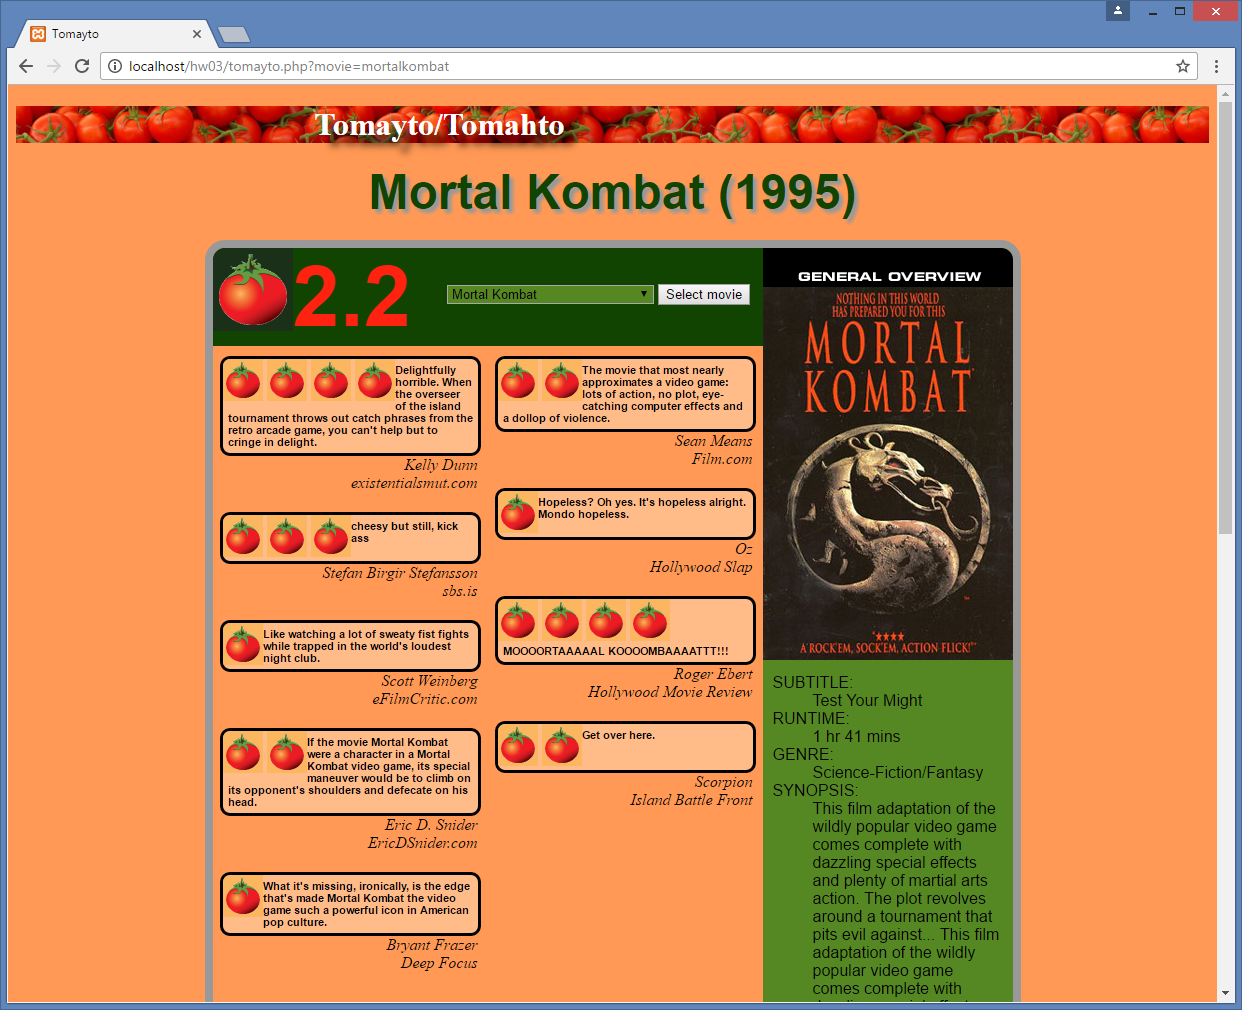
\includegraphics[width=\textwidth]{images/screenshot.png}
  \caption{Screenshot of final webpage.}
\label{screenshot}
\end{figure}

\end{document}
